\section{Method}
\label{sec:method}

In this section we propose a new method for automatically selecting good small multiple displays. Our approach takes three inputs from the analyst:
\begin{enumerate}
\item a visualization which the user wants to partition into a small multiple display,
\item a quality measure defined on this visualization type that captures patterns of interest to the user, and
\item a list of potential partitioning variables.
\end{enumerate}
The output is a scoring of the small multiple displays produced by each partitioning variable.

In the following section, we describe desirable properties for small multiple displays that we use to motivate our approach. The next section describes our method in the context of a running example. We then discuss some straightforward extensions to our basic approach.

\subsection{Goodness-of-Split Criteria}
To guide our approach, we formulated the following four goodness criteria. Partitioning variables should be chosen such that the resulting small multiple displays are:
\begin{itemize}
\item \emph{Visually rich}: We want small multiple displays that convey rich visual patterns, as captured by the quality metric provided by the analyst. In contrast to statistical methods, such as ANOVA, which are based on relatively simple summary metrics with closed-form distributions under some assumptions, most visualization quality metrics involve complicated processing and do not follow a known distribution.

\item \emph{Informative}: The purpose of a small multiple display is to help explain patterns in the input visualization. We want to prefer partitioning variables that add information to the display, supporting the user in their analysis. Partitions that randomly split the data are not useful since they don't contain any more information than the original plot.

\item \emph{Well-supported}: For some data sets, particularly those with outliers or with a small number of data points, strong visual patterns can occur by chance. These spurious patterns are misleading; they appear informative, but are not. We would like to detect and downweight such spurious patterns, guiding analysts to more robust results.

\item \emph{Parsimonious}: A small multiple display with many partitions can be very difficult to read and understand. All things being equal, we want to favor splitting into as few plots as possible, while still providing an informative display.
\end{itemize}



\subsection{Algorithm}

\begin{figure*}
 \centering 
    \begin{subfigure}[t]{1.35in}
        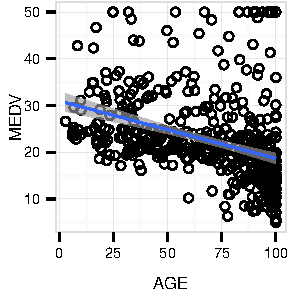
\includegraphics[width=1.35in]{images/AGE-MEDV.pdf}
        \caption{Input}
        \label{fig:method_original}
    \end{subfigure}
    \begin{subfigure}[t]{1.5in}
 	 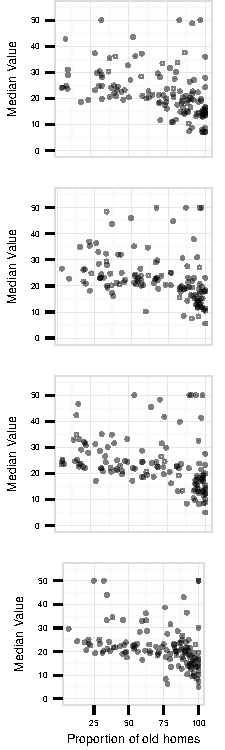
\includegraphics[width=1.5in]{images/randCluster.pdf}
	 \label{fig:method_random}
 	\caption{}
    \end{subfigure}
    \begin{subfigure}[t]{1.5in}
  	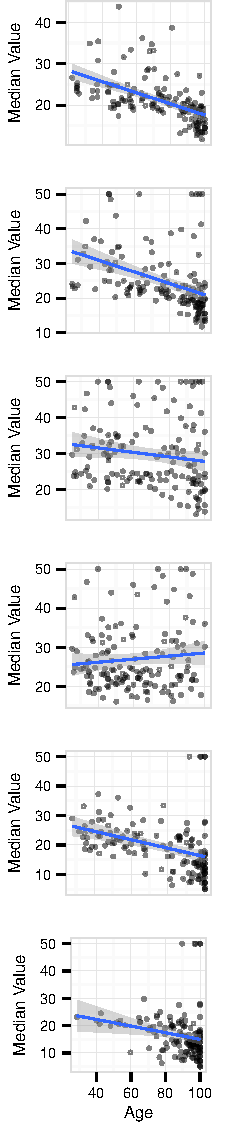
\includegraphics[width=1.5in]{images/RM.pdf}
	\caption{}
	 \label{fig:method_actual}
    \end{subfigure}
     \begin{subfigure}[t]{1.9in}
 	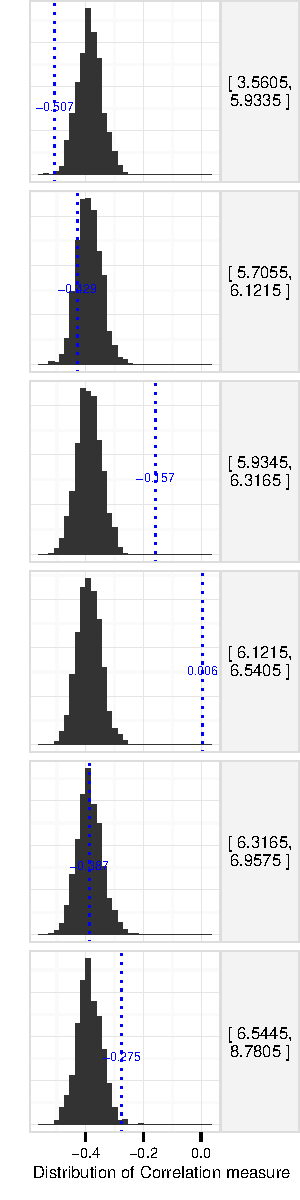
\includegraphics[width=1.9in]{images/hist-RM.pdf}
	\caption{}
	 \label{fig:method_dist}
     \end{subfigure}
   \caption{Illustration of our method of evaluating small multiple displays. (a) Partitions determined by the levels of Industrial growth. (b)Randomly permuted partitions of data. (c) Distribution of Monotonic measures for randomly permuted partitions. The overlaid blue lines are the corresponding Monotonic measures of the partitions determined by Industrial growth in (a).}
\end{figure*}

%Given a user-selected set of response variables, we want to automatically find a good Split respecting the criteria outlined above. This process of selecting a good Split, adding a conditioning variable to explain the visual structure in a set of data observations when we have many potential such variables, is akin to the model selection process. We evaluate the ``model" a Split determines based not only on the quality of the interesting patterns in partitions, but also, on the simplicity or size of the collection of partitions. Model selection is commonly employed in statistics and data mining to pick a statistical model that fits a sample of data, such as curve fitting or clustering. However, applying such a methodology with cognostics or visual pattern measures studied in the information visualization community has not been explored. We describe an algorithm to apply cognostics to do model selection where a model is determined as the addition of an explanatory variable to a selected set of response variables. 

Our approach is based on a permutation test, which is a non-parametric statistical significance test where the distribution of a test statistic under the null hypothesis is determined by computing the test statistic on rearrangements of the observed data points. Here, we find the statistical significance of a particular small multiple display using a cognostic as the test statistic. This allows us to evaluate small multiples for patterns not due to chance, so we can automatically find good small multiples according to our criteria above.

To understand how this algorithm works, consider the example in Figure~\ref{fig:method_original} showing the user-selected interesting bivariate relationship between the median value of owner-occupied homes in $\$1000's$ and the proportion of owner-occupied units built prior to 1940. This dataset~\cite{Harrison1978}  contains information collected by the U.S Census Service concerning housing in the area of Boston Massachusetts. We see that as the age of houses increases, their median value decreases.

Central to our approach is the use of a cognostic~\cite{Tukey1982,Tukey1985}, a diagnostic measure to evaluate the usefulness of a data. Tukey proposed such the use of such quality measures to filter the large number of views of a high-dimensional dataset. Here, a cognostic is an independent, substitutable piece of the approach and its choice is based on the user's task and interest. For our example with the Boston housing dataset, we use the Monotonic scagnostic~\cite{Wilkinson2005} as our cognostic.

Let the partitioning variable $d_p$ create $k$ partitions with sizes $\left\{ {s_1, s_2,...,s_k}\right\}$. We compute the cognostic on each of these $k$ partitions to get a set of cognostics $\left\{ {c_1, c_2,...,c_k}\right\}$. Figure~\ref{fig:method_actual} shows the small multiple resulting from using the "Industry" variable, which denotes the proportion of non-retail business acres per town, to partition the original view. The partitions, going from the top of the bottom, have sizes $\left\{ {69, 72, 76, 62, 38,189}\right\}$ and Monotonic measures $\left\{ {0.015, 0.0, 0.043, 0.244, 0.168, 0.052}\right\}$. This partitioning reveals the interesting effect of industrial growth on the value of older houses. With low levels of industrial growth, there is no clear relationship between the age and median house value but as the levels of industrial growth increase in a neighborhood, older houses decrease in value.

Then, we generate a random permutation of the original data into $k$ partitions of the same sizes $\left\{ {s_1, s_2,...,s_k}\right\}$ as seen in Figure~\ref{fig:method_random}. We use permutation sampling as we assume our dataset is representative of the population and do not need to compensate, via bootstrapping, for the assumption that it represents a sample from a larger, unexamined population. (NEED MORE HERE). We compute the Monotonic measure on each of these $k$ random partitions. Then we generate $r$ such randomly permuted partitions and corresponding sets of measures to create $k$ distributions of cognostics as seen in Figure~\ref{fig:method_dist}. 

The generated cognostic distributions function as reference "null distributions" and we apply a non-parametric significance test to determine how significant the difference is between the partitions determined by a particular variable and random partitions. The z-score from Chebyshev's inequality is as follows:
$$\sum_{i=1}^n \frac{(x_i-\mu_i)^2}{\sigma_i^2}$$
where $x_i$ is the score of the i-th partition and $\mu_i$ and $\sigma_i$ are the mean and standard deviation of the cognostic measures for the i-th partition for the randomly-generated partitions. We then combine the $k$ z-scores to produce one value that serves as a ranking metric for a particular partitioning dimension. We take the maximum of the z-scores from the partitions which ranks the Industry variable at the top of all the other partitioning choices with a score of $4.144$. Combining scores with the sum or the mean would not penalize dimensions with many partitions. (NEED MORE HERE)

\subsection{Handling Continuous Partitioners}
Determining discrete splits for a categorical variable is trivial as the observations are naturally partitioned into subsets for each discrete choice the variable offers. For continuous variables, discrete partitions can be created through a binning technique. There are various binning techniques that split a continuous range into disjoint intervals~\cite{Freedman1981,Scott2009} employed in histograms. An alternative binning strategy is one with overlapping bins of roughly equal count called shingles~\cite{Becker1996 ?Cleveland book first??}. The overlap of the intervals increases the resolution with which we can study conditional independence in the same way that moving averages increase the resolution of local behavior at each time point. 
%Figure~\ref{fig:shingles} shows such �moving snapshots� of the data across the range of the partitioning variable.

\subsection{Multiple Partitioners}
%NOT SURE IF THIS FITS HERE STILL OR SHOULD BE IN THE DISCUSSION
Small multiples or trellis plots facet a single view into multiple views combining partitioning variables using cross and nest operators~\cite{Wilkinson2005GG,Stolte2002}. Our algorithm could be used to progressively pick variables to partition on in the transition from a large single view~\cite{van2013} to informative small multiples.


